\section{Challenges and Opportunities}\label{sec:challenges}

What becomes a challenge is when all branches of a PHYSLITE file need to be read including branches with custom objects and when systematics need to be handled.
As columnar analysis processes events in batches, this requires that ATLAS Combined Performance (CP) tools and algorithms must also be able to operate in batches.
The current model for CP tools is to operate on the ATLAS xAOD event data model (EDM) for all the calculations per event and then to write the systematics to disk for future access.
This process is I/O intensive, but has been computationally efficient for the current ATLAS analysis model.
The challenge for a fully columnar CP tool framework is to adapt to the on-the-fly computation of the columnar paradigm --- furthering the ``trade disk for compute'' strategy --- while still being performant enough to not be a bottleneck.

This refactoring process ongoing in the ATLAS Analysis Model Group (AMG) has also offered design improvement opportunities to create more Pythonic end-user APIs for the ATLAS CP tools.
As seen in~\Cref{fig:columnar_cp_tools_diagram}, creating Pythonic APIs for users allows for integration with the broader scientific Python ecosystem, but through efficient binding layers all data can be efficiently passed through to the \texttt{C++} CP tools for efficient computation, and then the results can be exposed to the users again.
By using \texttt{nanobind}~\cite{nanobind} --- next generation \texttt{C++}-to-Python bindings --- it becomes possible to have zero-copy operations to and from $n$-dimensional array libraries in Python, including those which support hardware accelerators like GPUs, and full design control of the high-level user API.
The API design ability is quite powerful, as it allows for unification of interfaces to CP tools without requiring individual CP tools to redesign their APIs.

As a first (\texttt{v1}) prototype of this capability, external zero-copy \texttt{nanobind} Python bindings to a columnar implementation of the ATLAS Egamma CP tool were created to compute on-the-fly systematics for $m_{ee}$.
Uproot was used to load PHYSLITE ATLAS simulation into Awkward arrays, and event selections were applied with Coffea.
The standalone Pythonic interface to the Egamma tool, \texttt{atlascp.EgammaTools}, was initialized and then systematics were computed on-the-fly while being scaled out with \texttt{dask-awkward}~\cite{dask_awkward_2024} on the University of Chciago ATLAS Analysis Facility.
The results are plotted in~\Cref{fig:Zee_mc_systematics}.
This \texttt{v1} prototype established foundations of what was possible with new tooling and that Pythonic interfaces to CP tools could be written without large amounts of work or deep knowledge of underlying CP tool design.
This was promising, but additional work was needed to achieve necessary performance required for use.
Though as there was no ``zero action'' option --- some amount of research was required to determine the viability of the proposed design --- this prototype was valuable.

Following this work, a \texttt{v2} ``Columnar Athena'' prototype~\cite{columnar_athena} has been started to expand the scope of the work.
This moves the development of the columnar CP tools and interfaces from standalone examples into the ATLAS Athena framework and migrates the ATLAS CP tools to a columnar backend with breaking the existing workflows using the EDM models.
It additionally adds infrastructure support for development of columnar analysis tools by adding \texttt{nanobind} to the ATLAS Externals tooling distributed as part of the ATLAS Athena Analysis Releases.
While currently under active development, the \texttt{v2} prototype will allow for full scale integration and performance tests of the columnar CP tools and interfaces.

\begin{figure}
    \centering
    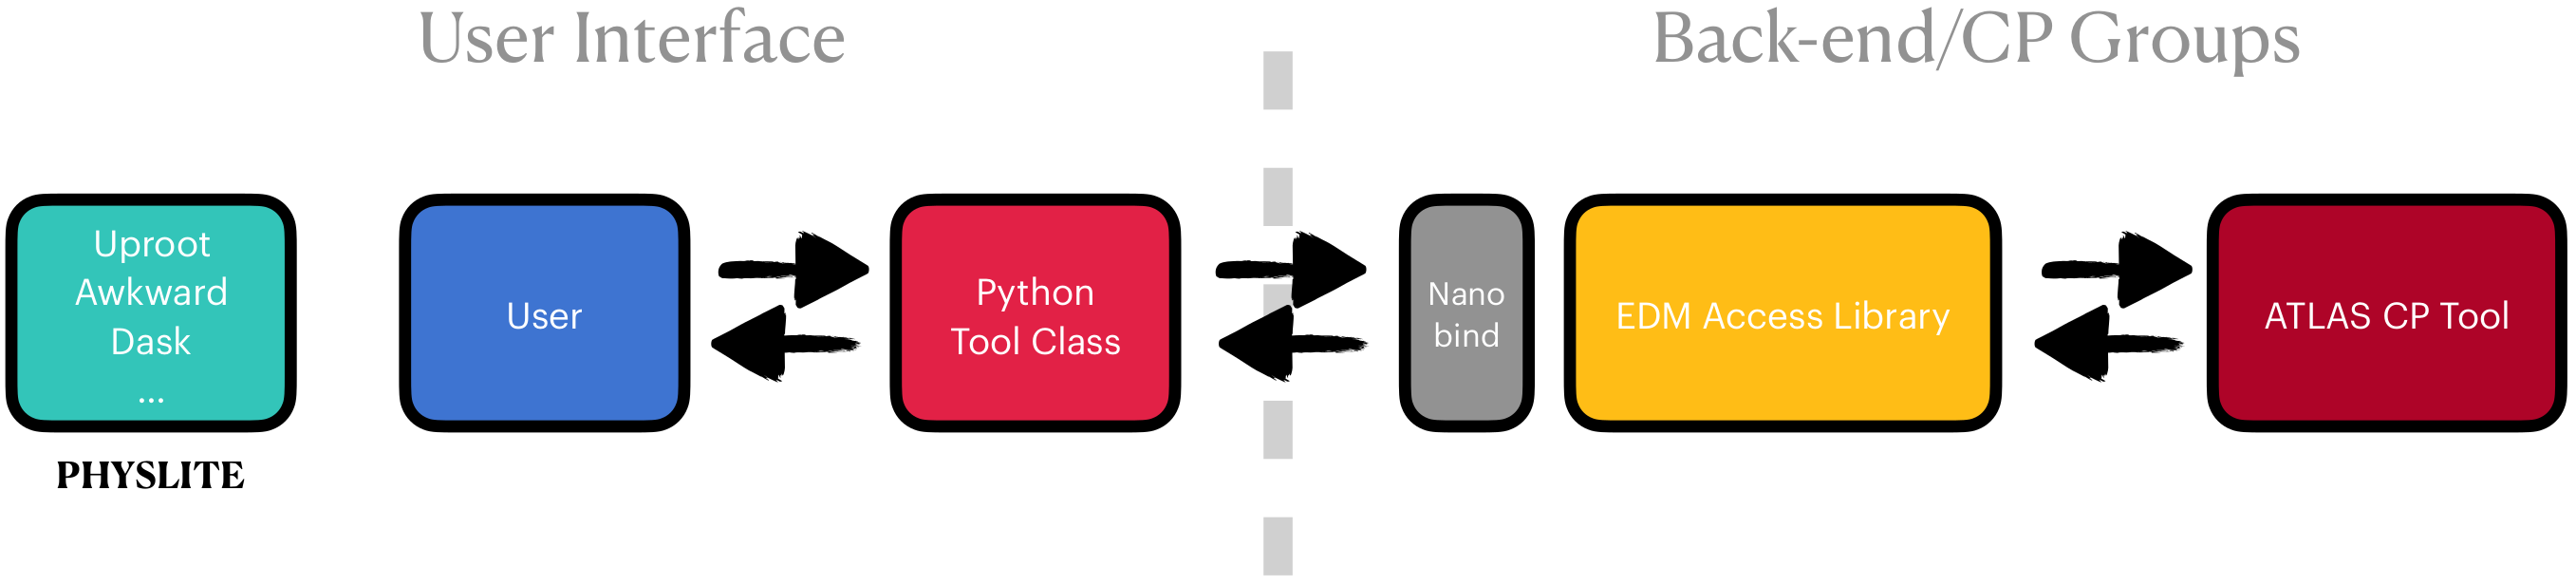
\includegraphics[width=\textwidth]{columnar_cp_tools_diagram.png}
    \caption{X~\cite{Vigl:ACAT_2024}.}
    \label{fig:columnar_cp_tools_diagram}
\end{figure}

\begin{figure}
    \centering
    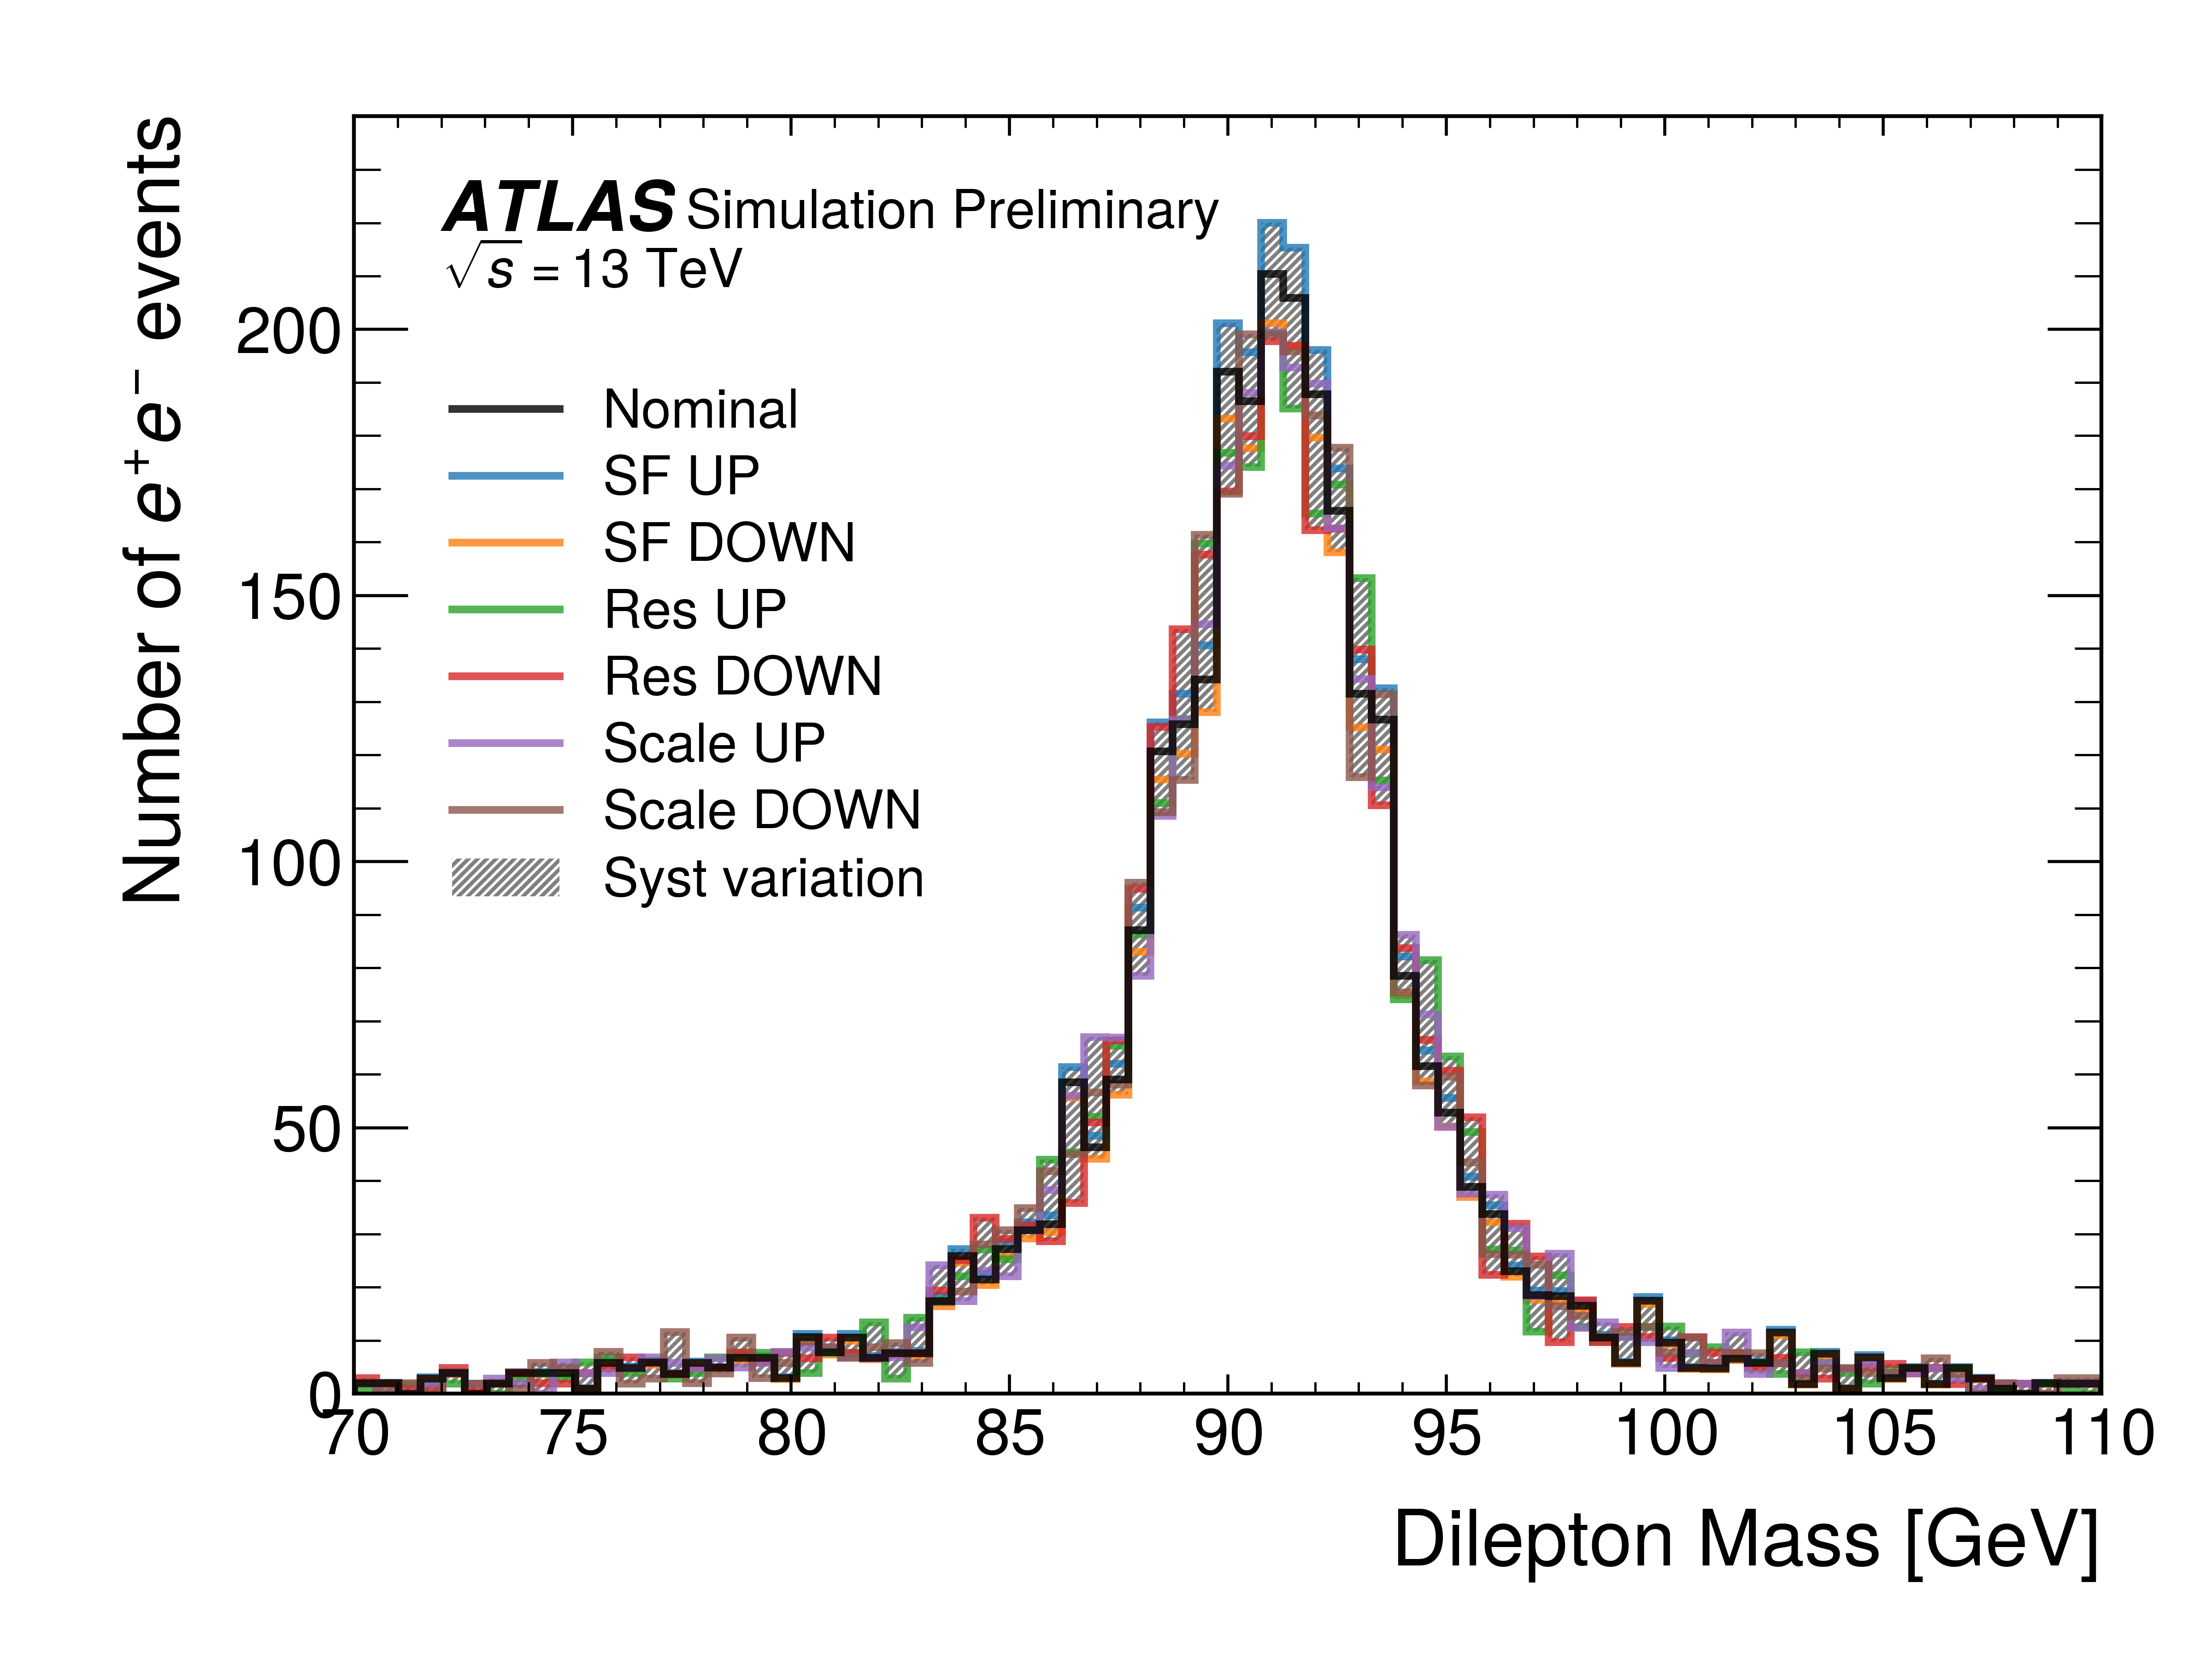
\includegraphics[width=0.7\textwidth]{Zee_mc_systematics.png}
    \caption{Selected $m_{ee}$ under on-the-fly computed systematic variations of electron reconstruction efficiency and corrections~\cite{Vigl:ACAT_2024}.}
    \label{fig:Zee_mc_systematics}
\end{figure}
